\begin{frame}{Probabilistic Modeling}

%source:https://texample.net/tikz/examples/connecting-text-and-graphics/


\begin{columns}
    \begin{column}{0.48\textwidth}
        \centering
        \tiny
        \begin{equation*}
            \tiny
            \label{eqn:gaussian}
            \alpha_{ij} = \sum_{r=0}^{R} \eta^r w_{ij}^r \, y_{ij}^r + \epsilon_{ij}, \qquad \epsilon_{ij} \sim \mathcal{N}(0, \sigma_{ij}^2)
        \end{equation*}
        \begin{equation*}
        \eta^r w_{ij}^r = \eta^r \frac{\text{total num. groups}}{\text{num. similar groups}}, \,  i<j
        \\
        \eta^rw_{ij}^r = \eta^r \frac{\text{total num. groups}}{\text{num. dissimilar groups}}, \,  i>j
        \end{equation*}\\
        \vspace{0.3cm}
        
        %considering that one of the pairs is the attention test we have 10*9/2 FPC, which gives 5 similar pairs and 39 dissimilar pairs. 39+5 = 44, 44+1(attention pair) = 45 =10*9/2
        % idea is to have top and bottom sum up to 1
        % \fontsize{4.5}{4.5}\selectfont
        \tiny
        \begin{bmatrix}
        0 & 0 & 0 & 0 & 0 & 0 & \frac{5}{5} & 0 & 0 & 0 \\ 
        \frac{5}{39} & 0 & 0 & 0 & 0 & 0 & 0 & \frac{5}{5} & 0 & 0  \\ 
        \vdots & \vdots & \vdots & \vdots & \vdots & \vdots & \vdots & \vdots & \vdots & \vdots \\
        \frac{5}{39} & \frac{5}{39} & \frac{5}{39} & \frac{5}{39} & \frac{5}{39} & 0 & \frac{5}{39} & \frac{5}{39} & 0 &  0 \\ 
        \frac{5}{39} & \frac{5}{39} & 0 & \frac{5}{39} & \frac{5}{39} & \frac{5}{39} & \frac{5}{39} & \frac{5}{39} & \frac{5}{39} & 0 \\ 
        \end{bmatrix}

        
    \end{column}
    \begin{column}{0.48\textwidth}
        \tikzstyle{background grid}=[draw, black!50,step=.5cm]
        \begin{tikzpicture}%[show background grid]
            % Put the graphic inside a node. This makes it easy to place the
            % graphic and to draw on top of it. 
            % The above right option is used to place the lower left corner
            % of the image at the (0,0) coordinate. 
            \node [inner sep=0pt,above right] 
                {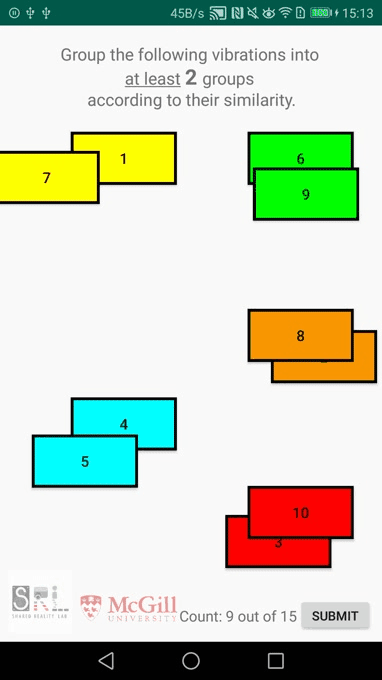
\includegraphics[width=4cm]{Images/3.png}};
            % show origin
            % \fill (0,0) circle (2pt);
            % define destination coordinates
            % \path (2.5,5.3) coordinate (im69)
            %       (2.3,1.3) coordinate (im310);
        \end{tikzpicture}
    \end{column}
\end{columns}

% define overlays
% Note the use of the overlay option. This is required when 
% you want to access nodes in different pictures.
% \begin{tikzpicture}[overlay]
        % \path[<-,green,thick] (s-69) edge [bend left] (im69);
        % \path[<-,red,thick] (s-310) edge [bend right] (im310);
% \end{tikzpicture}


\end{frame}